\documentclass{standalone}
\usepackage{tikz}
\usetikzlibrary{patterns, positioning}

\begin{document}
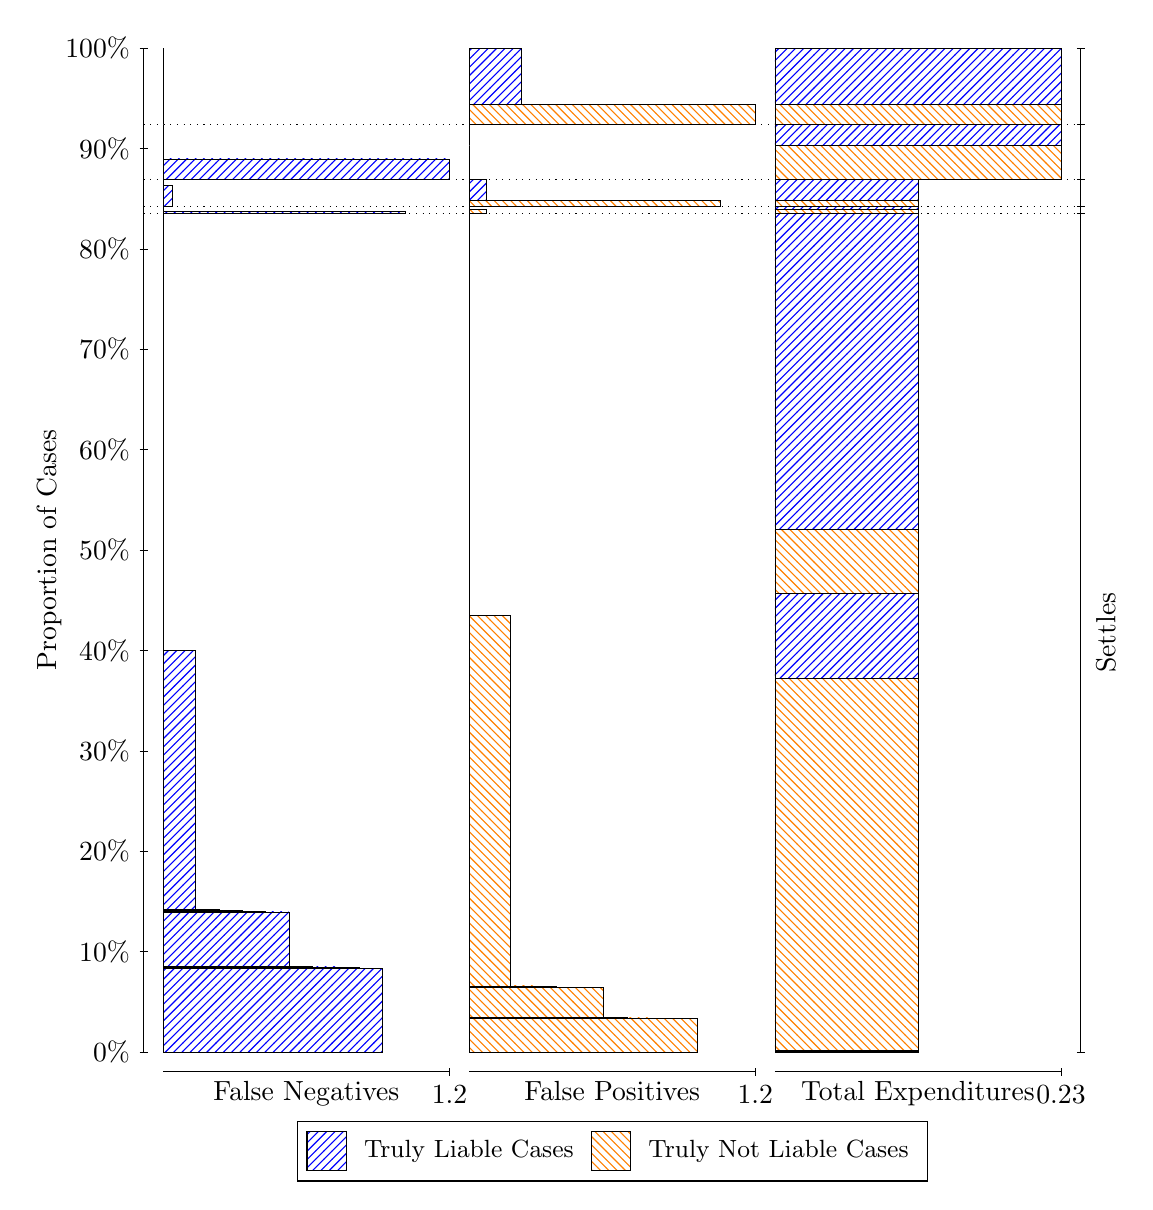
\begin{tikzpicture}
\draw[black, very thin] (1.5,1.75) -- (1.5,14.5);
\node[rotate=90, anchor=center] at (0.3, 8.125) {Proportion of Cases};
\draw[black, very thin] (1.45,1.75) -- (1.55,1.75);
\node[anchor=east] at (1.45, 1.75) {0\%};
\draw[black, very thin] (1.45,3.025) -- (1.55,3.025);
\node[anchor=east] at (1.45, 3.025) {10\%};
\draw[black, very thin] (1.45,4.3) -- (1.55,4.3);
\node[anchor=east] at (1.45, 4.3) {20\%};
\draw[black, very thin] (1.45,5.575) -- (1.55,5.575);
\node[anchor=east] at (1.45, 5.575) {30\%};
\draw[black, very thin] (1.45,6.85) -- (1.55,6.85);
\node[anchor=east] at (1.45, 6.85) {40\%};
\draw[black, very thin] (1.45,8.125) -- (1.55,8.125);
\node[anchor=east] at (1.45, 8.125) {50\%};
\draw[black, very thin] (1.45,9.4) -- (1.55,9.4);
\node[anchor=east] at (1.45, 9.4) {60\%};
\draw[black, very thin] (1.45,10.675) -- (1.55,10.675);
\node[anchor=east] at (1.45, 10.675) {70\%};
\draw[black, very thin] (1.45,11.95) -- (1.55,11.95);
\node[anchor=east] at (1.45, 11.95) {80\%};
\draw[black, very thin] (1.45,13.225) -- (1.55,13.225);
\node[anchor=east] at (1.45, 13.225) {90\%};
\draw[black, very thin] (1.45,14.5) -- (1.55,14.5);
\node[anchor=east] at (1.45, 14.5) {100\%};

\draw[black, very thin] (13.4,1.75) -- (13.4,14.5);
\draw[black, very thin] (13.35,1.75) -- (13.45,1.75);
\node[anchor=west] at (13.35, 1.75) {};
\draw[black, very thin] (13.35,12.396) -- (13.45,12.396);
\node[anchor=west] at (13.35, 12.396) {};
\draw[black, very thin] (13.35,12.485) -- (13.45,12.485);
\node[anchor=west] at (13.35, 12.485) {};
\draw[black, very thin] (13.35,12.832) -- (13.45,12.832);
\node[anchor=west] at (13.35, 12.832) {};
\draw[black, very thin] (13.35,13.527) -- (13.45,13.527);
\node[anchor=west] at (13.35, 13.527) {};
\draw[black, very thin] (13.35,14.5) -- (13.45,14.5);
\node[anchor=west] at (13.35, 14.5) {};

\draw[black, very thin, pattern color=blue, pattern=north east lines] (1.75,1.75) rectangle (4.5306,2.809);
\draw[black, very thin, pattern color=blue, pattern=north east lines] (1.75,2.809) rectangle (4.234,2.8195);
\draw[black, very thin, pattern color=blue, pattern=north east lines] (1.75,2.8195) rectangle (3.9374,2.8304);
\draw[black, very thin, pattern color=blue, pattern=north east lines] (1.75,2.8304) rectangle (3.6408,2.8415);
\draw[black, very thin, pattern color=blue, pattern=north east lines] (1.75,2.8415) rectangle (3.3442,3.5292);
\draw[black, very thin, pattern color=blue, pattern=north east lines] (1.75,3.5292) rectangle (3.0476,3.5377);
\draw[black, very thin, pattern color=blue, pattern=north east lines] (1.75,3.5377) rectangle (2.751,3.5466);
\draw[black, very thin, pattern color=blue, pattern=north east lines] (1.75,3.5466) rectangle (2.4544,3.556);
\draw[black, very thin, pattern color=blue, pattern=north east lines] (1.75,3.556) rectangle (2.1578,6.8506);
\draw[black, very thin, pattern color=orange, pattern=north west lines] (1.75,6.8506) rectangle (1.75,12.396);
\draw[black, very thin, pattern color=blue, pattern=north east lines] (1.75,12.396) rectangle (4.8272,12.428);
\draw[black, very thin, pattern color=orange, pattern=north west lines] (1.75,12.428) rectangle (1.75,12.485);
\draw[black, very thin, pattern color=blue, pattern=north east lines] (1.75,12.485) rectangle (1.8612,12.755);
\draw[black, very thin, pattern color=orange, pattern=north west lines] (1.75,12.755) rectangle (1.75,12.832);
\draw[black, very thin, pattern color=blue, pattern=north east lines] (1.75,12.832) rectangle (5.3833,13.093);
\draw[black, very thin, pattern color=orange, pattern=north west lines] (1.75,13.093) rectangle (1.75,13.527);
\draw[black, very thin, pattern color=orange, pattern=north west lines] (1.75,13.527) rectangle (1.75,13.789);
\draw[black, very thin, pattern color=blue, pattern=north east lines] (1.75,13.789) rectangle (1.75,14.5);
\draw[black, very thin, pattern color=orange, pattern=north west lines] (5.6333,1.75) rectangle (8.5252,2.1761);
\draw[black, very thin, pattern color=orange, pattern=north west lines] (5.6333,2.1761) rectangle (8.2286,2.1793);
\draw[black, very thin, pattern color=orange, pattern=north west lines] (5.6333,2.1793) rectangle (7.932,2.1824);
\draw[black, very thin, pattern color=orange, pattern=north west lines] (5.6333,2.1824) rectangle (7.6354,2.1853);
\draw[black, very thin, pattern color=orange, pattern=north west lines] (5.6333,2.1853) rectangle (7.3388,2.5655);
\draw[black, very thin, pattern color=orange, pattern=north west lines] (5.6333,2.5655) rectangle (7.0422,2.5656);
\draw[black, very thin, pattern color=orange, pattern=north west lines] (5.6333,2.5656) rectangle (7.0422,2.5736);
\draw[black, very thin, pattern color=orange, pattern=north west lines] (5.6333,2.5736) rectangle (6.7456,2.5816);
\draw[black, very thin, pattern color=orange, pattern=north west lines] (5.6333,2.5816) rectangle (6.449,2.5893);
\draw[black, very thin, pattern color=orange, pattern=north west lines] (5.6333,2.5893) rectangle (6.1524,7.2958);
\draw[black, very thin, pattern color=blue, pattern=north east lines] (5.6333,7.2958) rectangle (5.6333,12.396);
\draw[black, very thin, pattern color=orange, pattern=north west lines] (5.6333,12.396) rectangle (5.8558,12.453);
\draw[black, very thin, pattern color=blue, pattern=north east lines] (5.6333,12.453) rectangle (5.6333,12.485);
\draw[black, very thin, pattern color=orange, pattern=north west lines] (5.6333,12.485) rectangle (8.8218,12.562);
\draw[black, very thin, pattern color=blue, pattern=north east lines] (5.6333,12.562) rectangle (5.8558,12.832);
\draw[black, very thin, pattern color=orange, pattern=north west lines] (5.6333,12.832) rectangle (5.6333,13.265);
\draw[black, very thin, pattern color=blue, pattern=north east lines] (5.6333,13.265) rectangle (5.6333,13.527);
\draw[black, very thin, pattern color=orange, pattern=north west lines] (5.6333,13.527) rectangle (9.2667,13.789);
\draw[black, very thin, pattern color=blue, pattern=north east lines] (5.6333,13.789) rectangle (6.3007,14.5);
\draw[black, very thin, pattern color=orange, pattern=north west lines] (9.5167,1.75) rectangle (11.333,1.7577);
\draw[black, very thin, pattern color=blue, pattern=north east lines] (9.5167,1.7577) rectangle (11.333,1.7683);
\draw[black, very thin, pattern color=orange, pattern=north west lines] (9.5167,1.7683) rectangle (11.333,6.4908);
\draw[black, very thin, pattern color=blue, pattern=north east lines] (9.5167,6.4908) rectangle (11.333,7.5718);
\draw[black, very thin, pattern color=orange, pattern=north west lines] (9.5167,7.5718) rectangle (11.333,8.3873);
\draw[black, very thin, pattern color=blue, pattern=north east lines] (9.5167,8.3873) rectangle (11.333,12.396);
\draw[black, very thin, pattern color=orange, pattern=north west lines] (9.5167,12.396) rectangle (11.333,12.453);
\draw[black, very thin, pattern color=blue, pattern=north east lines] (9.5167,12.453) rectangle (11.333,12.485);
\draw[black, very thin, pattern color=orange, pattern=north west lines] (9.5167,12.485) rectangle (11.333,12.562);
\draw[black, very thin, pattern color=blue, pattern=north east lines] (9.5167,12.562) rectangle (11.333,12.832);
\draw[black, very thin, pattern color=orange, pattern=north west lines] (9.5167,12.832) rectangle (13.15,13.265);
\draw[black, very thin, pattern color=blue, pattern=north east lines] (9.5167,13.265) rectangle (13.15,13.527);
\draw[black, very thin, pattern color=orange, pattern=north west lines] (9.5167,13.527) rectangle (13.15,13.789);
\draw[black, very thin, pattern color=blue, pattern=north east lines] (9.5167,13.789) rectangle (13.15,14.5);
\draw[black, dotted] (1.5,12.396) -- (13.4,12.396);
\draw[black, dotted] (1.5,12.485) -- (13.4,12.485);
\draw[black, dotted] (1.5,12.832) -- (13.4,12.832);
\draw[black, dotted] (1.5,13.527) -- (13.4,13.527);
\draw[black, very thin] (1.75,1.5) -- (5.3833,1.5);
\node[anchor=north] at (3.5667, 1.5) {False Negatives};
\draw[black, very thin] (5.3833,1.45) -- (5.3833,1.55);
\node[anchor=north] at (5.3833, 1.45) {1.2};

\draw[black, very thin] (5.6333,1.5) -- (9.2667,1.5);
\node[anchor=north] at (7.45, 1.5) {False Positives};
\draw[black, very thin] (9.2667,1.45) -- (9.2667,1.55);
\node[anchor=north] at (9.2667, 1.45) {1.2};

\draw[black, very thin] (9.5167,1.5) -- (13.15,1.5);
\node[anchor=north] at (11.333, 1.5) {Total Expenditures};
\draw[black, very thin] (13.15,1.45) -- (13.15,1.55);
\node[anchor=north] at (13.15, 1.45) {0.23};

\node[black, centered, rotate=90] at (13.72, 7.0732) {Settles};





\draw (7.449999999999999,1.5) node[draw=none] (baseCoordinate) {};
\begin{scope}[align=center]
        \matrix[scale=0.5, draw=black, below=0.5cm of baseCoordinate, nodes={draw}, column sep=0.1cm]{
            \node[rectangle, draw, minimum width=0.5cm, minimum height=0.5cm, pattern=north east lines, pattern color=blue] {}; &
            \node[draw=none, font=\small] (B) {Truly Liable Cases}; &
            \node[rectangle, draw, minimum width=0.5cm, minimum height=0.5cm, pattern=north west lines, pattern color=orange] {}; &
            \node[draw=none, font=\small] (B) {Truly Not Liable Cases}; \\
            };
\end{scope}

\end{tikzpicture}
\end{document}